% IEEE Conference Paper - KiwiDB Implementation
% Compile with: pdflatex kiwidb-implementation-paper.tex

\documentclass[conference]{IEEEtran}

\usepackage{amsmath,amssymb,amsfonts}
\usepackage{algorithmic}
\usepackage{graphicx}
\usepackage{textcomp}
\usepackage{xcolor}
\usepackage{listings}
\usepackage{booktabs}
\usepackage{multirow}
\usepackage{url}
\usepackage{hyperref}
\usepackage{float}
\usepackage{enumitem}
\usepackage{tikz}
\usetikzlibrary{arrows.meta, positioning, shapes.geometric, fit, calc, decorations.pathreplacing}

\lstset{
  basicstyle=\footnotesize\ttfamily,
  breaklines=true,
  frame=single,
  numbers=left,
  numberstyle=\tiny,
  tabsize=2,
  captionpos=b
}

\begin{document}

\title{KiwiDB: An Async-Native Log-Structured Merge Tree Key-Value Store with Parallel Flush and Subprocess Compaction}

\author{
\IEEEauthorblockN{Chaitanya Paraskar}
\IEEEauthorblockA{Department of Computer Engineering \\
University of Pune \\
Pune, India \\
chaitanya.paraskar@example.com}
% Add additional authors as needed
}

\maketitle

\begin{abstract}
Log-Structured Merge Trees (LSM trees) are the dominant write-optimized storage engine architecture, underpinning systems such as LevelDB, RocksDB, and Apache Cassandra. However, existing implementations are written in C/C++ with synchronous APIs, making them incompatible with modern asynchronous application frameworks. This paper presents KiwiDB, an LSM tree key-value store implemented from scratch in Python~3.12+. KiwiDB introduces three design innovations: (1)~an async-native API where the event loop never blocks on disk I/O; (2)~a parallel flush pipeline with event-chain ordered commits that achieves concurrent SSTable writes while preserving strict FIFO ordering; and (3)~subprocess-based compaction that bypasses CPython's Global Interpreter Lock (GIL) for true write-path isolation. The engine employs a hybrid L0-tiering / L1-leveling compaction strategy, a concurrent skip list with lock-free reads, data-derived bloom filter sizing, and a three-tier block cache. Compared with the stock LevelDB design, KiwiDB reduces flush-time write amplification by $10\times$ and provides built-in observability through a FastAPI REST interface and a React web dashboard. The system comprises approximately 6,600 lines of type-checked Python with 211 tests across 25 modules.
\end{abstract}

\begin{IEEEkeywords}
LSM tree, key-value store, async I/O, compaction, skip list, bloom filter, write-ahead log, Python, storage engine
\end{IEEEkeywords}

% ============================================================
\section{Introduction}
% ============================================================

With the rapid growth of web applications and cloud computing, key-value (KV) stores have become a critical component of modern data infrastructure. A KV store maps a set of keys to associated values and can be considered a distributed hash table. Without having to provide features usually required for a relational database system, KV stores offer higher performance, better scalability, and more availability~\cite{leavitt2010}. They play a central role in data centers supporting Internet-scale services, including BigTable~\cite{chang2008} at Google, Cassandra~\cite{cassandra} at Facebook, and Dynamo~\cite{decandia2007} at Amazon.

The B+ tree is a common structure used in traditional databases, because its high fanout reduces the number of I/O operations for a query. However, it is highly inefficient for random insertions and updates. When there are intensive mutations, B+ trees lead to a large number of costly disk seeks and significantly degraded performance. The Log-Structured Merge Tree (LSM tree)~\cite{oneil1996} addresses this by transforming random writes into sequential writes: incoming data is sorted in an in-memory buffer and flushed to storage as a whole when the buffer is full. Many popular KV stores adopt this design, including BigTable~\cite{chang2008}, Cassandra~\cite{cassandra}, HBase~\cite{hbase}, and LevelDB~\cite{leveldb}.

Despite the maturity of these systems, we observe two limitations that motivate this work:

\textbf{(1) Synchronous APIs.} LevelDB and RocksDB~\cite{rocksdb} expose blocking C++ interfaces. Modern Python applications (FastAPI, aiohttp) run on \texttt{asyncio} event loops. Integrating a synchronous storage engine requires thread-pool wrappers that add latency, complexity, and concurrency bugs. To the best of our knowledge, no existing LSM implementation offers a natively asynchronous API.

\textbf{(2) Opaque internals.} Production engines prioritize throughput over observability. Inspecting memtable state, bloom filter hit rates, compaction progress, or SSTable layouts requires external tooling. Internal design decisions are documented sparsely, making these systems difficult to learn from.

To address these limitations, we present KiwiDB, an LSM tree key-value store implemented from scratch in Python~3.12+. The contributions of this work are:

\begin{itemize}[leftmargin=*]
    \item KiwiDB provides an \textbf{async-native API} where all public operations (\texttt{put}, \texttt{get}, \texttt{delete}, \texttt{flush}, \texttt{close}) are async coroutines. WAL fsync, SSTable flush, and compaction execute off the event loop via \texttt{asyncio.to\_thread()} and \texttt{ProcessPoolExecutor}.

    \item We design a \textbf{parallel flush pipeline} that writes multiple SSTables concurrently while preserving strict FIFO commit ordering via an \texttt{asyncio.Event} chain. We prove its crash-safety properties and analyze failure propagation.

    \item Compaction merges run in \textbf{subprocess workers} via \texttt{ProcessPoolExecutor}, bypassing CPython's GIL to achieve true CPU parallelism with zero impact on the write path.

    \item We adopt a \textbf{hybrid L0-tiering / L1-leveling} compaction strategy that reduces write amplification by $10\times$ compared to LevelDB's pure leveling, and implement a \textbf{concurrent skip list} with lock-free reads and per-node write locking.

    \item We provide a \textbf{built-in observability layer} with a FastAPI REST interface, a React web dashboard, and live log streaming via WebSocket --- making the engine's internal state fully inspectable in real time.
\end{itemize}

The remainder of this paper is organized as follows. Section~2 provides background on LevelDB's architecture and CPython's GIL. Section~3 describes how we extend the LSM design with our proposed techniques. Section~4 discusses implementation-specific details and Python-specific challenges. We describe related work in Section~5, followed by conclusions in Section~6.

% ============================================================
\section{Background}
\label{sec:background}
% ============================================================

In order to present the details of our design, we first review the architecture of LevelDB, the canonical LSM tree implementation. Then we describe CPython's Global Interpreter Lock, which motivates several of our design decisions.

\subsection{LevelDB Architecture}

LevelDB~\cite{leveldb} is an open-source KV store that originated from Google's BigTable~\cite{chang2008}. It is a widely studied implementation of the LSM tree~\cite{leveldb, wang2014locs}. Figure~\ref{fig:leveldb-arch} illustrates its architecture, which consists of two MemTables in main memory and a set of SSTables on disk, along with auxiliary files such as the Manifest and the write-ahead log.

% --- Figure 1: LevelDB Architecture ---
\begin{figure}[t]
\centering
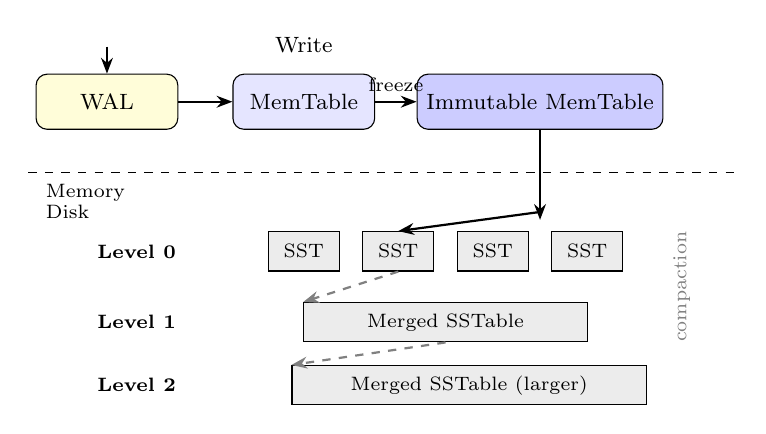
\begin{tikzpicture}[
    box/.style={draw, rounded corners, minimum width=1.8cm, minimum height=0.7cm, font=\footnotesize},
    sst/.style={draw, fill=gray!15, minimum width=0.9cm, minimum height=0.5cm, font=\scriptsize},
    arr/.style={-{Stealth[length=2mm]}, thick},
    label/.style={font=\scriptsize\itshape},
    >=Stealth
]
% Memory region
\node[box, fill=blue!10] (mt) at (0, 3.5) {MemTable};
\node[box, fill=blue!20] (imt) at (3, 3.5) {Immutable MemTable};
\node[box, fill=yellow!15] (wal) at (-2.5, 3.5) {WAL};

% Arrows
\node[font=\footnotesize, above=0.15cm of mt] {Write};
\draw[arr] (mt) -- node[above, font=\scriptsize] {freeze} (imt);
\draw[arr] (-2.5, 4.2) -- (wal);
\draw[arr] (wal) -- (mt);

% Disk region
\draw[dashed] (-3.5, 2.6) -- (5.5, 2.6);
\node[font=\scriptsize, anchor=west] at (-3.4, 2.35) {Memory};
\node[font=\scriptsize, anchor=west] at (-3.4, 2.85) {};
\node[font=\scriptsize, anchor=west] at (-3.4, 2.1) {Disk};

% L0
\draw[arr] (imt) -- (3, 2.0) node[right, font=\scriptsize] {};
\node[font=\scriptsize\bfseries, anchor=east] at (-1.5, 1.6) {Level 0};
\node[sst] (l0a) at (0, 1.6) {SST};
\node[sst] (l0b) at (1.2, 1.6) {SST};
\node[sst] (l0c) at (2.4, 1.6) {SST};
\node[sst] (l0d) at (3.6, 1.6) {SST};
\draw[arr] (3, 2.1) -- (l0b.north);

% L1
\node[font=\scriptsize\bfseries, anchor=east] at (-1.5, 0.7) {Level 1};
\node[sst, minimum width=3.6cm] (l1) at (1.8, 0.7) {Merged SSTable};

% L2
\node[font=\scriptsize\bfseries, anchor=east] at (-1.5, -0.1) {Level 2};
\node[sst, minimum width=4.5cm] (l2) at (2.1, -0.1) {Merged SSTable (larger)};

% Compaction arrows
\draw[arr, dashed, gray] (l0b.south) -- (l1.north west);
\draw[arr, dashed, gray] (l1.south) -- (l2.north west);
\node[font=\scriptsize, gray, rotate=90] at (4.8, 1.15) {compaction};

\end{tikzpicture}
\caption{Architecture of LevelDB. Writes go to the WAL and MemTable. When the MemTable is full, it becomes an Immutable MemTable and is flushed to Level~0. Compaction merges SSTables across levels.}
\label{fig:leveldb-arch}
\end{figure}

\textbf{Write path.} When the user inserts a KV pair, it is first appended to the write-ahead log (WAL) for durability, then inserted into the MemTable, a sorted in-memory structure. When the MemTable reaches its size limit, it is converted to a read-only Immutable MemTable. A new MemTable is created for incoming writes. A background thread flushes the Immutable MemTable to disk as a Sorted String Table (SSTable). Deletes are a special case: a deletion marker (tombstone) is stored.

\textbf{Level organization.} SSTables are organized into levels. Level~0 is produced directly from MemTable flushes and may contain overlapping key ranges. Levels~1 and above have non-overlapping key ranges within each level. Each level has a size limit that grows exponentially: Level~1 holds up to 10\,MB, Level~2 up to 100\,MB, and so on.

\textbf{Compaction.} When the total size of Level~$L$ exceeds its limit, the compaction thread picks one SSTable from Level~$L$ and all overlapping SSTables from Level~$L{+}1$, merges them, and produces new Level~$L{+}1$ files. This eliminates overwritten values, drops tombstones, and ensures that fresher data resides in lower levels.

\textbf{Read path.} A \texttt{get(key)} request searches the MemTable, then the Immutable MemTable, then SSTables from Level~0 upward until a match is found. Since lower levels contain fresher data, the first match is authoritative. A Bloom filter~\cite{bloom1970} in each SSTable reduces unnecessary I/O by quickly ruling out files that do not contain the requested key.

\textbf{Limitations.} Two aspects of LevelDB's design are relevant to this work. First, there is only \textbf{one} Immutable MemTable and \textbf{one} background thread for flush and compaction. If the MemTable fills while the Immutable MemTable is still being flushed, writes are blocked. Second, the API is entirely synchronous --- every operation blocks the calling thread until completion.

\subsection{CPython's Global Interpreter Lock}

CPython, the reference Python implementation, uses a Global Interpreter Lock (GIL) that allows only one thread to execute Python bytecode at a time~\cite{python-gil}. This has two consequences for a storage engine:

\begin{enumerate}[leftmargin=*]
    \item \textbf{I/O-bound work is unaffected}: Threads release the GIL during system calls (\texttt{read}, \texttt{write}, \texttt{fsync}), so I/O-bound operations like WAL append and SSTable reads achieve true concurrency.
    \item \textbf{CPU-bound work is serialized}: A compaction merge that iterates millions of records in Python is CPU-bound and cannot benefit from multi-threading. True parallelism requires a separate \emph{process} with its own GIL.
\end{enumerate}

Table~\ref{tab:gil-impact} summarizes the impact on each engine component and the concurrency strategy KiwiDB adopts.

\begin{table}[t]
\centering
\caption{Impact of CPython's GIL on engine components and the concurrency strategy adopted by KiwiDB.}
\label{tab:gil-impact}
\begin{tabular}{@{}llll@{}}
\toprule
\textbf{Component} & \textbf{Bound} & \textbf{GIL Impact} & \textbf{KiwiDB Strategy} \\
\midrule
MemTable insert & CPU & Serialized & Sync (fast, $\mu$s) \\
WAL fsync & I/O & GIL released & \texttt{to\_thread()} \\
SSTable read & I/O & GIL released & \texttt{mmap} (zero-copy) \\
SSTable write & I/O & GIL released & Async parallel \\
Compaction & CPU & \textbf{Serialized} & \textbf{Subprocess} \\
\bottomrule
\end{tabular}
\end{table}

% ============================================================
\section{Design and Implementation}
\label{sec:design}
% ============================================================

In this section we first introduce the architectural overview of KiwiDB. Then we describe each subsystem extension over the classical LevelDB design: the async-native write and read paths, the concurrent skip list, the parallel flush pipeline, the hybrid compaction strategy, and the observability layer.

\subsection{Overall Architecture}

Figure~\ref{fig:kiwidb-arch} shows the overall architecture of KiwiDB, organized into a strict layered dependency model. The system consists of seven tiers, from leaf modules (Tier~0: types, CRC, UUID) up to the top-level engine coordinator (Tier~6: \texttt{LSMEngine}). No module imports from a tier above it, preventing circular dependencies and enabling each tier to be tested in isolation.

% --- Figure 2: KiwiDB Overall Architecture ---
\begin{figure}[t]
\centering
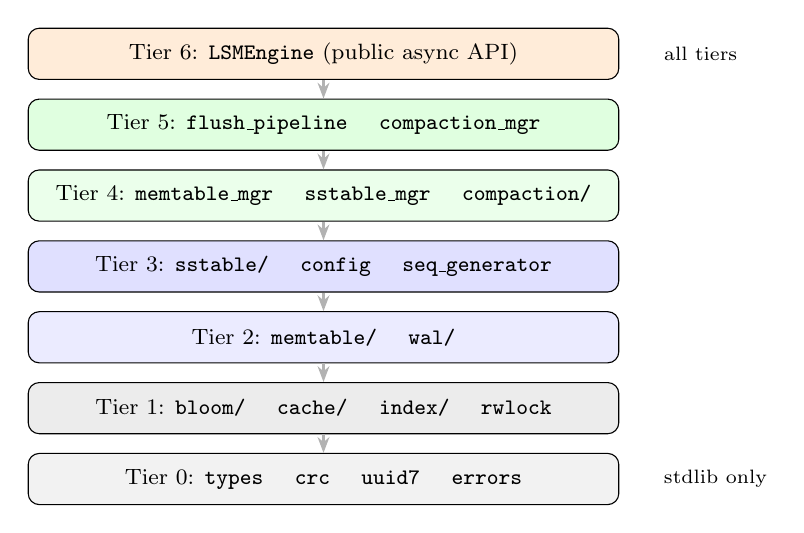
\begin{tikzpicture}[
    tier/.style={draw, rounded corners, minimum width=7.5cm, minimum height=0.65cm, font=\footnotesize, fill=#1},
    arr/.style={-{Stealth[length=2mm]}, thick},
    >=Stealth
]
% Tiers (bottom to top)
\node[tier=gray!10] (t0) at (0, 0) {Tier 0: \texttt{types} \quad \texttt{crc} \quad \texttt{uuid7} \quad \texttt{errors}};
\node[tier=gray!15] (t1) at (0, 0.9) {Tier 1: \texttt{bloom/} \quad \texttt{cache/} \quad \texttt{index/} \quad \texttt{rwlock}};
\node[tier=blue!8] (t2) at (0, 1.8) {Tier 2: \texttt{memtable/} \quad \texttt{wal/}};
\node[tier=blue!12] (t3) at (0, 2.7) {Tier 3: \texttt{sstable/} \quad \texttt{config} \quad \texttt{seq\_generator}};
\node[tier=green!8] (t4) at (0, 3.6) {Tier 4: \texttt{memtable\_mgr} \quad \texttt{sstable\_mgr} \quad \texttt{compaction/}};
\node[tier=green!12] (t5) at (0, 4.5) {Tier 5: \texttt{flush\_pipeline} \quad \texttt{compaction\_mgr}};
\node[tier=orange!15] (t6) at (0, 5.4) {Tier 6: \texttt{LSMEngine} (public async API)};

% Dependency arrows
\foreach \upper/\lower in {t1/t0, t2/t1, t3/t2, t4/t3, t5/t4, t6/t5} {
    \draw[arr, gray!60] (\upper.south) -- (\lower.north);
}

% Labels
\node[font=\scriptsize, anchor=west] at (4.2, 0) {stdlib only};
\node[font=\scriptsize, anchor=west] at (4.2, 5.4) {all tiers};

\end{tikzpicture}
\caption{KiwiDB layered architecture. Each tier depends only on tiers below it. The engine at Tier~6 is a thin coordinator.}
\label{fig:kiwidb-arch}
\end{figure}

As shown in Figure~\ref{fig:kiwidb-arch}, the software is composed of six subsystems: the Write-Ahead Log (WAL), MemTable with concurrent skip list, SSTable storage with bloom filter and sparse index, flush pipeline, compaction engine, and observability layer. The engine coordinates these subsystems through managers at Tiers~4--5.

Table~\ref{tab:system-spec} lists the software specification of KiwiDB.

\begin{table}[t]
\centering
\caption{KiwiDB software specification.}
\label{tab:system-spec}
\begin{tabular}{@{}ll@{}}
\toprule
\textbf{Property} & \textbf{Value} \\
\midrule
Language & Python 3.12+ \\
Lines of code & $\sim$6,600 (engine) \\
Test suite & 211 tests across 25 modules \\
Type checking & mypy strict + basedpyright strict \\
Linting & ruff + bandit (security) \\
Build system & uv + setuptools \\
Web framework & FastAPI + Vite/React \\
Key dependencies & msgpack, mmh3, structlog, cachetools \\
\bottomrule
\end{tabular}
\end{table}

\subsection{Async-Native Write Path}

All writes in KiwiDB follow the same atomic path under a single lock. The key invariant is \textbf{durability before visibility}: the WAL is fsynced before the memtable is updated. Figure~\ref{fig:write-path} illustrates this four-step sequence.

% --- Figure 3: Write Path ---
\begin{figure}[t]
\centering
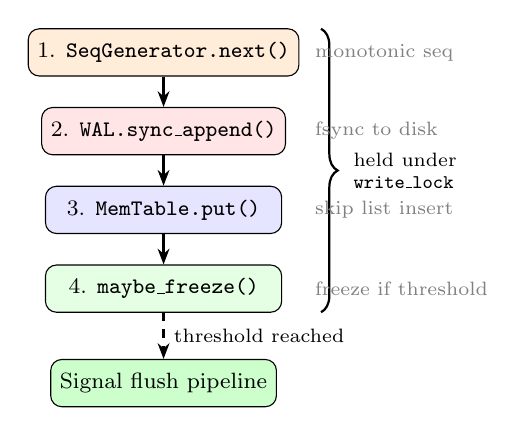
\begin{tikzpicture}[
    step/.style={draw, rounded corners, minimum width=3cm, minimum height=0.6cm, font=\footnotesize, fill=#1},
    arr/.style={-{Stealth[length=2mm]}, thick},
    >=Stealth
]
\node[step=orange!15] (s1) at (0, 4.0) {1. \texttt{SeqGenerator.next()}};
\node[step=red!10] (s2) at (0, 3.0) {2. \texttt{WAL.sync\_append()}};
\node[step=blue!10] (s3) at (0, 2.0) {3. \texttt{MemTable.put()}};
\node[step=green!10] (s4) at (0, 1.0) {4. \texttt{maybe\_freeze()}};

\draw[arr] (s1) -- (s2);
\draw[arr] (s2) -- (s3);
\draw[arr] (s3) -- (s4);

% Lock brace
\draw[decorate, decoration={brace, amplitude=6pt, mirror}, thick] (2.0, 0.7) -- (2.0, 4.3) node[midway, right=8pt, font=\scriptsize, align=left] {held under\\\texttt{write\_lock}};

% Annotations
\node[font=\scriptsize, anchor=west, gray] at (1.8, 4.0) {monotonic seq};
\node[font=\scriptsize, anchor=west, gray] at (1.8, 3.0) {fsync to disk};
\node[font=\scriptsize, anchor=west, gray] at (1.8, 2.0) {skip list insert};
\node[font=\scriptsize, anchor=west, gray] at (1.8, 1.0) {freeze if threshold};

% Freeze branch
\node[step=green!20, minimum width=2.5cm] (freeze) at (0, -0.2) {Signal flush pipeline};
\draw[arr, dashed] (s4) -- node[right, font=\scriptsize] {threshold reached} (freeze);

\end{tikzpicture}
\caption{KiwiDB write path. All four steps execute atomically under \texttt{write\_lock}. The WAL is fsynced (Step~2) before the memtable is updated (Step~3), ensuring durability before visibility.}
\label{fig:write-path}
\end{figure}

\textbf{Step 1: Sequence generation.} \texttt{SeqGenerator.next()} atomically increments a monotonic counter under \texttt{threading.Lock}. This sequence number serves as the MVCC version --- higher values indicate newer data.

\textbf{Step 2: WAL durability.} The entry is serialized using msgpack and framed as \texttt{[4B~length][payload][4B~CRC32]}. Two operation types are supported: \texttt{PUT}~(op=1) and \texttt{DELETE}~(op=2). The file descriptor is fsynced before returning. This is the most expensive step, but it guarantees that even if the process crashes immediately after \texttt{put()} returns, the entry is recoverable.

\textbf{Step 3: MemTable insert.} The KV pair is inserted into the active skip list (described in Section~\ref{sec:skiplist}).

\textbf{Step 4: Conditional freeze.} If the active memtable exceeds its threshold, it is frozen into an \texttt{ImmutableMemTable}, pushed to the immutable queue, and the flush pipeline is signaled. Table~\ref{tab:freeze-thresholds} shows the freeze conditions.

\begin{table}[t]
\centering
\caption{MemTable freeze thresholds by environment.}
\label{tab:freeze-thresholds}
\begin{tabular}{@{}llll@{}}
\toprule
\textbf{Mode} & \textbf{Condition} & \textbf{Default} & \textbf{Config Key} \\
\midrule
Dev & entry count $\geq$ limit & 10 entries & \texttt{max\_memtable\_entries} \\
Prod & byte size $\geq$ limit & 64\,MB & \texttt{max\_memtable\_size\_mb} \\
\bottomrule
\end{tabular}
\end{table}

\textbf{Lock ordering.} KiwiDB enforces a strict ordering --- \texttt{write\_lock} $\rightarrow$ \texttt{wal\_lock} --- to prevent deadlock. The write path holds \texttt{write\_lock} while calling \texttt{sync\_append()}, which internally acquires \texttt{wal\_lock}. Reversing this order would deadlock.

\textbf{Delete vs.\ Put.} A \texttt{delete(key)} follows the identical path but writes \texttt{OpType.DELETE} with a tombstone sentinel value \texttt{b"\textbackslash x00\_\_tomb\_\_\textbackslash x00"}. The tombstone propagates through flush and compaction until garbage-collected.

\subsection{Read Path}

Figure~\ref{fig:read-path} illustrates the read path. Reads scan data sources from newest to oldest, returning the first match with the highest sequence number. Crucially, \textbf{no write locks are acquired} --- reads are non-blocking.

% --- Figure 4: Read Path ---
\begin{figure}[t]
\centering
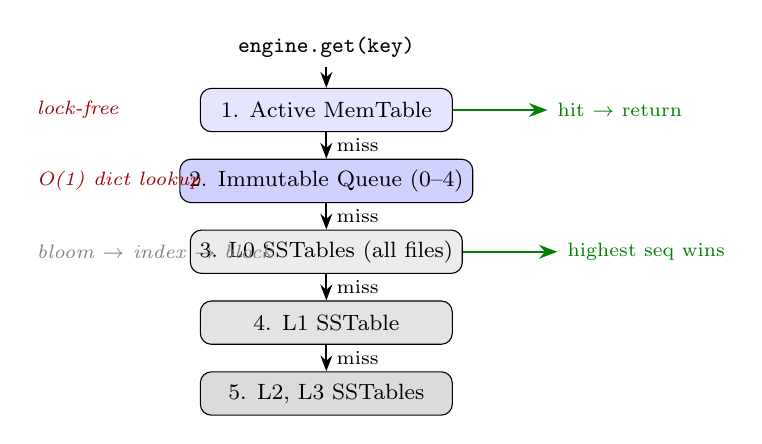
\begin{tikzpicture}[
    src/.style={draw, rounded corners, minimum width=3.2cm, minimum height=0.55cm, font=\footnotesize, fill=#1},
    arr/.style={-{Stealth[length=2mm]}, thick},
    >=Stealth
]
\node[font=\footnotesize\bfseries] at (0, 5.0) {\texttt{engine.get(key)}};

\node[src=blue!10] (s1) at (0, 4.2) {1. Active MemTable};
\node[src=blue!18] (s2) at (0, 3.3) {2. Immutable Queue (0--4)};
\node[src=gray!15] (s3) at (0, 2.4) {3. L0 SSTables (all files)};
\node[src=gray!22] (s4) at (0, 1.5) {4. L1 SSTable};
\node[src=gray!28] (s5) at (0, 0.6) {5. L2, L3 SSTables};

\draw[arr] (0, 4.75) -- (s1);
\draw[arr] (s1) -- node[right, font=\scriptsize] {miss} (s2);
\draw[arr] (s2) -- node[right, font=\scriptsize] {miss} (s3);
\draw[arr] (s3) -- node[right, font=\scriptsize] {miss} (s4);
\draw[arr] (s4) -- node[right, font=\scriptsize] {miss} (s5);

% Hit annotation
\draw[-{Stealth}, thick, green!50!black] (s1.east) -- ++(1.2, 0) node[right, font=\scriptsize] {hit $\rightarrow$ return};
\draw[-{Stealth}, thick, green!50!black] (s3.east) -- ++(1.2, 0) node[right, font=\scriptsize] {highest seq wins};

% Lookup detail for SSTable
\node[font=\scriptsize, anchor=west, gray] at (-3.8, 2.4) {\textit{bloom $\rightarrow$ index $\rightarrow$ block}};

% Lock-free annotation
\node[font=\scriptsize, anchor=west, red!60!black] at (-3.8, 4.2) {\textit{lock-free}};
\node[font=\scriptsize, anchor=west, red!60!black] at (-3.8, 3.3) {\textit{O(1) dict lookup}};

\end{tikzpicture}
\caption{KiwiDB read path. Data sources are checked newest-first. MemTable lookup is lock-free. Each SSTable uses a bloom~$\rightarrow$~index~$\rightarrow$~block pipeline. The first match with the highest sequence number wins.}
\label{fig:read-path}
\end{figure}

\textbf{Step 1:} The active memtable is searched via $O(\log n)$ lock-free skip list traversal.

\textbf{Step 2:} The immutable queue (up to 4 frozen snapshots) is scanned newest-first. Each lookup is $O(1)$ via an internal dictionary index.

\textbf{Step 3:} All L0 SSTables are checked because their key ranges overlap. For each file, the lookup pipeline is: \textit{bloom filter} (rule out absent keys) $\rightarrow$ \textit{sparse index bisect} (find candidate block) $\rightarrow$ \textit{block scan} (sequential scan within block). The result with the highest sequence number across all L0 files is kept.

\textbf{Steps 4--5:} L1--L3 each have at most one SSTable. The same bloom $\rightarrow$ index $\rightarrow$ block pipeline applies, but only one file per level needs checking.

\textbf{Tombstone resolution:} After finding a result from any source, if the value equals the tombstone sentinel, the key has been deleted --- the engine returns \texttt{None}.

\textbf{Example.} Suppose a user writes \texttt{put("x", "v1")} with seq=5, then \texttt{put("x", "v2")} with seq=8, then the memtable flushes to L0. A \texttt{get("x")} first checks the (now empty) active memtable, then the immutable queue, then L0. In L0, the SSTable contains both records; the one with seq=8 wins. The engine returns \texttt{"v2"}.

\subsection{Concurrent Skip List}
\label{sec:skiplist}

The memtable is backed by a concurrent skip list with 16 levels and promotion probability $p = 0.5$. Figure~\ref{fig:skiplist} shows the node structure and concurrency model.

% --- Figure 5: Skip List ---
\begin{figure}[t]
\centering
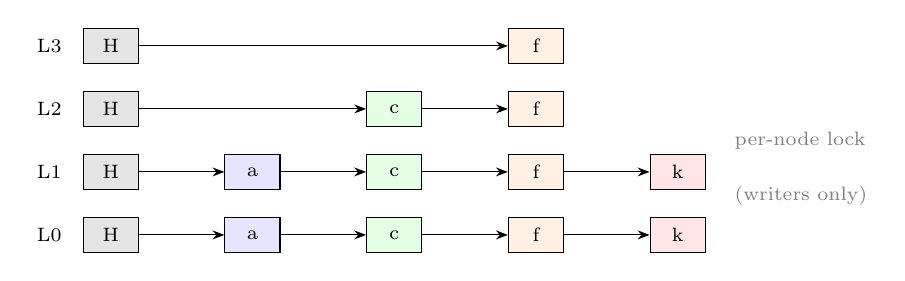
\begin{tikzpicture}[
    node/.style={draw, minimum width=0.7cm, minimum height=0.45cm, font=\scriptsize},
    head/.style={draw, fill=gray!20, minimum width=0.7cm, minimum height=0.45cm, font=\scriptsize},
    arr/.style={-{Stealth[length=1.5mm]}},
    >=Stealth
]
% Head
\node[head] (h3) at (0, 2.4) {H};
\node[head] (h2) at (0, 1.6) {H};
\node[head] (h1) at (0, 0.8) {H};
\node[head] (h0) at (0, 0) {H};

% Node A (key="a")
\node[node, fill=blue!10] (a1) at (1.8, 0.8) {a};
\node[node, fill=blue!10] (a0) at (1.8, 0) {a};

% Node C (key="c")
\node[node, fill=green!10] (c2) at (3.6, 1.6) {c};
\node[node, fill=green!10] (c1) at (3.6, 0.8) {c};
\node[node, fill=green!10] (c0) at (3.6, 0) {c};

% Node F (key="f")
\node[node, fill=orange!10] (f3) at (5.4, 2.4) {f};
\node[node, fill=orange!10] (f2) at (5.4, 1.6) {f};
\node[node, fill=orange!10] (f1) at (5.4, 0.8) {f};
\node[node, fill=orange!10] (f0) at (5.4, 0) {f};

% Node K (key="k")
\node[node, fill=red!10] (k1) at (7.2, 0.8) {k};
\node[node, fill=red!10] (k0) at (7.2, 0) {k};

% Level 3 arrows
\draw[arr] (h3) -- (f3);

% Level 2 arrows
\draw[arr] (h2) -- (c2);
\draw[arr] (c2) -- (f2);

% Level 1 arrows
\draw[arr] (h1) -- (a1);
\draw[arr] (a1) -- (c1);
\draw[arr] (c1) -- (f1);
\draw[arr] (f1) -- (k1);

% Level 0 arrows
\draw[arr] (h0) -- (a0);
\draw[arr] (a0) -- (c0);
\draw[arr] (c0) -- (f0);
\draw[arr] (f0) -- (k0);

% Level labels
\node[font=\scriptsize, anchor=east] at (-0.5, 2.4) {L3};
\node[font=\scriptsize, anchor=east] at (-0.5, 1.6) {L2};
\node[font=\scriptsize, anchor=east] at (-0.5, 0.8) {L1};
\node[font=\scriptsize, anchor=east] at (-0.5, 0) {L0};

% Lock annotation
\node[font=\scriptsize, anchor=west, gray] at (7.8, 1.2) {per-node lock};
\node[font=\scriptsize, anchor=west, gray] at (7.8, 0.5) {(writers only)};

\end{tikzpicture}
\caption{Concurrent skip list with four keys. Each node has per-node \texttt{threading.Lock} for writers. Readers traverse lock-free by checking GIL-atomic \texttt{fully\_linked} and \texttt{marked} boolean flags.}
\label{fig:skiplist}
\end{figure}

Each node stores: \texttt{key}, \texttt{seq} (MVCC version), \texttt{timestamp\_ms}, \texttt{value}, \texttt{forward[]} (one pointer per level), a per-node \texttt{threading.Lock}, and two boolean flags: \texttt{marked} (logical deletion) and \texttt{fully\_linked} (visibility).

\textbf{Writer protocol.} Writers lock only the predecessor nodes at the insertion boundary. Two concurrent inserts with disjoint keys do not contend. The protocol is: (1)~top-down traversal to find predecessors and successors, (2)~lock predecessors, (3)~validate they are still correct, (4)~create the node and link at level~0, (5)~link at higher levels and set \texttt{fully\_linked = True}, (6)~release locks.

\textbf{Lock-free readers.} Readers perform a top-down traversal checking the \texttt{fully\_linked} and \texttt{marked} flags. Under CPython, single-attribute reads on Python objects are GIL-atomic --- no torn reads occur. This makes reader traversal effectively lock-free without CAS instructions.

Table~\ref{tab:skiplist-comparison} compares the concurrency models of the three engines.

\begin{table}[t]
\centering
\caption{MemTable concurrency model comparison.}
\label{tab:skiplist-comparison}
\begin{tabular}{@{}llll@{}}
\toprule
\textbf{Engine} & \textbf{Structure} & \textbf{Write} & \textbf{Read} \\
\midrule
LevelDB & Skip list & Global mutex & Serialized \\
RocksDB & Skip list & Lock-free (CAS) & Lock-free \\
KiwiDB & Skip list & Per-node locks & Lock-free (GIL) \\
\bottomrule
\end{tabular}
\end{table}

\subsection{SSTable Format}

Each SSTable is a directory containing four files, as shown in Table~\ref{tab:sstable-layout}. The presence of \texttt{meta.json} is the completeness signal: if it is missing, the SSTable is considered incomplete (e.g., crash during write) and is ignored on recovery.

\begin{table}[t]
\centering
\caption{SSTable directory layout.}
\label{tab:sstable-layout}
\begin{tabular}{@{}lp{5.5cm}@{}}
\toprule
\textbf{File} & \textbf{Purpose} \\
\midrule
\texttt{data.bin} & Sorted KV records grouped into $\sim$4\,KB blocks \\
\texttt{index.bin} & Sparse index: first key per block $\rightarrow$ byte offset \\
\texttt{filter.bin} & Bloom filter bit array + header \\
\texttt{meta.json} & Metadata; written \textbf{last} as completeness signal \\
\bottomrule
\end{tabular}
\end{table}

\textbf{Record encoding.} Each record uses the binary format shown in Figure~\ref{fig:record-format}. The CRC32 covers the entire record for integrity verification.

% --- Figure 6: Record Format ---
\begin{figure}[t]
\centering
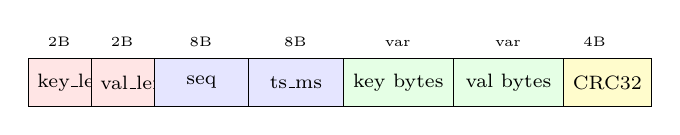
\begin{tikzpicture}[
    field/.style={draw, minimum height=0.6cm, font=\scriptsize, fill=#1, anchor=west},
]
\node[field=red!10, minimum width=0.8cm] (kl) at (0, 0) {key\_len};
\node[field=red!10, minimum width=0.8cm] (vl) at (0.8, 0) {val\_len};
\node[field=blue!10, minimum width=1.2cm] (sq) at (1.6, 0) {seq};
\node[field=blue!10, minimum width=1.2cm] (ts) at (2.8, 0) {ts\_ms};
\node[field=green!10, minimum width=1.4cm] (k) at (4.0, 0) {key bytes};
\node[field=green!10, minimum width=1.4cm] (v) at (5.4, 0) {val bytes};
\node[field=yellow!20, minimum width=0.8cm] (crc) at (6.8, 0) {CRC32};

% Size annotations
\node[font=\tiny, above=1pt] at (0.4, 0.3) {2B};
\node[font=\tiny, above=1pt] at (1.2, 0.3) {2B};
\node[font=\tiny, above=1pt] at (2.2, 0.3) {8B};
\node[font=\tiny, above=1pt] at (3.4, 0.3) {8B};
\node[font=\tiny, above=1pt] at (4.7, 0.3) {var};
\node[font=\tiny, above=1pt] at (6.1, 0.3) {var};
\node[font=\tiny, above=1pt] at (7.2, 0.3) {4B};

\end{tikzpicture}
\caption{SSTable record binary format. Key and value lengths are 2-byte big-endian unsigned integers. Sequence and timestamp are 8-byte big-endian signed integers.}
\label{fig:record-format}
\end{figure}

\textbf{Writer state machine.} The SSTable writer follows a strict lifecycle: \texttt{OPEN} $\rightarrow$ \texttt{put()$\times$N} $\rightarrow$ \texttt{finish()} $\rightarrow$ \texttt{DONE}. Keys must be in ascending order (enforced). \texttt{finish()} is async for L0 flushes (writing bloom and index concurrently via \texttt{asyncio.gather}), while \texttt{finish\_sync()} is synchronous for compaction subprocesses.

\textbf{Reader with mmap.} The reader uses memory-mapped I/O for zero-copy access to \texttt{data.bin}. Bloom filter and sparse index are loaded lazily on first \texttt{get()} and cached in the shared block cache.

\subsection{Bloom Filter with Data-Derived Sizing}

Unlike LevelDB and RocksDB, which use a fixed bits-per-key ratio, KiwiDB sizes each bloom filter using the \textbf{actual record count} $n$ at write time:

\begin{equation}
m = \left\lceil \frac{-n \cdot \ln p}{(\ln 2)^2} \right\rceil, \quad
k = \left\lceil \frac{m}{n} \cdot \ln 2 \right\rceil
\end{equation}

where $p$ is the target false positive rate, $m$ is the bit array size, and $k$ is the number of hash functions (MurmurHash3 with distinct seeds). Table~\ref{tab:bloom-comparison} shows the difference.

\begin{table}[t]
\centering
\caption{Bloom filter sizing comparison.}
\label{tab:bloom-comparison}
\begin{tabular}{@{}lll@{}}
\toprule
\textbf{Engine} & \textbf{Size Parameter} & \textbf{FPR Config} \\
\midrule
LevelDB & Fixed bits/key (default 10) & Fixed at creation \\
RocksDB & Fixed bits/key (configurable) & Per column family \\
KiwiDB & \textbf{Actual record count} & Per-env: 5\% dev, 1\% prod \\
\bottomrule
\end{tabular}
\end{table}

\textbf{Example.} If LevelDB uses 10 bits/key for an SSTable with 100 entries, it allocates 1,000 bits --- the same ratio it would use for 1M entries. KiwiDB computes the optimal bit count for exactly 100 entries at 1\% FPR: $m = \lceil -100 \cdot \ln(0.01) / (\ln 2)^2 \rceil = 959$ bits with $k = 7$ hash functions. Every SSTable gets a right-sized filter.

\subsection{Three-Tier Block Cache}

KiwiDB uses a three-tier LRU cache that serves data blocks, sparse indexes, and bloom filters with independent eviction policies. The tiered design reflects access patterns: bloom filters should remain resident (checked on every lookup), indexes are checked on positive bloom results, and data blocks are accessed only when the index indicates a candidate.

\begin{table}[t]
\centering
\caption{Block cache tier configuration.}
\label{tab:cache}
\begin{tabular}{@{}lccc@{}}
\toprule
\textbf{Tier} & \textbf{Key} & \textbf{Capacity} & \textbf{Eviction} \\
\midrule
Data blocks & offset $\geq 0$ & 256 entries & First (lowest priority) \\
Sparse indexes & offset = $-2$ & 64 entries & Medium \\
Bloom filters & offset = $-1$ & 64 entries & Last (highest priority) \\
\bottomrule
\end{tabular}
\end{table}

Each tier is backed by an independent \texttt{cachetools.LRUCache} with \texttt{threading.RLock} for thread safety. Cache entries persist across engine restarts: a new \texttt{SSTableReader} instance reuses cached bloom filters and indexes from a previous session.

\subsection{Parallel Flush Pipeline}
\label{sec:flush}

LevelDB uses a single background thread for flushing, which means that if the working MemTable fills while the Immutable MemTable is still being written, user writes are blocked. Wang et al.~\cite{wang2014locs} addressed this by increasing the number of Immutable MemTables and flushing them concurrently to separate SSD channels. KiwiDB adopts a similar insight at the software level --- multiple SSTables are written concurrently --- but must solve an additional problem: \textbf{commit ordering}.

On a multi-channel SSD, each SSTable lands on a separate channel and ordering is implicit. On a standard filesystem, KiwiDB must explicitly ensure that L0 files appear in oldest-first order, because the read path depends on this ordering. We solve this with an \textit{event-chain commit mechanism}.

\subsubsection{Event-Chain Mechanism}

Figure~\ref{fig:flush-pipeline} illustrates the mechanism with two workers. Each flush slot carries two \texttt{asyncio.Event} objects: \texttt{prev\_committed} (set by predecessor) and \texttt{my\_committed} (set by this slot).

% --- Figure 7: Parallel Flush Pipeline ---
\begin{figure}[t]
\centering
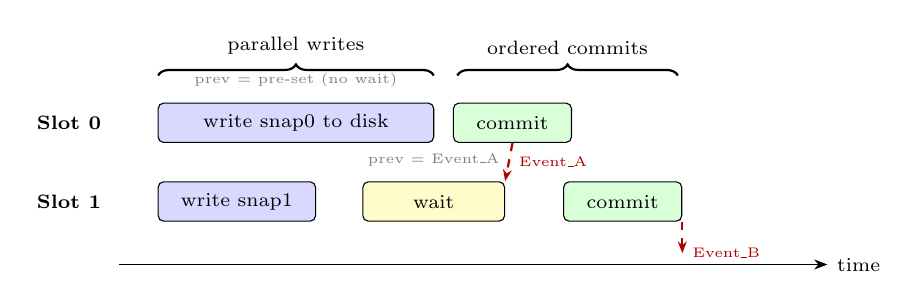
\begin{tikzpicture}[
    phase/.style={draw, minimum height=0.5cm, font=\scriptsize, rounded corners=2pt},
    arr/.style={-{Stealth[length=1.5mm]}, thick},
    >=Stealth
]
% Timeline
\draw[->] (-0.5, 0) -- (8.5, 0) node[right, font=\scriptsize] {time};

% Slot 0 (oldest snapshot)
\node[font=\scriptsize\bfseries, anchor=east] at (-0.6, 1.8) {Slot 0};
\node[phase, fill=blue!15, minimum width=3.5cm] (w0) at (1.75, 1.8) {write snap0 to disk};
\node[phase, fill=green!15, minimum width=1.5cm] (c0) at (4.5, 1.8) {commit};

% Slot 1 (newer snapshot)
\node[font=\scriptsize\bfseries, anchor=east] at (-0.6, 0.8) {Slot 1};
\node[phase, fill=blue!15, minimum width=2.0cm] (w1) at (1.0, 0.8) {write snap1};
\node[phase, fill=yellow!20, minimum width=1.8cm] (wait1) at (3.5, 0.8) {wait};
\node[phase, fill=green!15, minimum width=1.5cm] (c1) at (5.9, 0.8) {commit};

% Event arrows
\draw[arr, red!70!black, dashed] (c0.south) -- node[right, font=\tiny, red!70!black] {Event\_A} (wait1.north east);
\draw[arr, red!70!black, dashed] (c1.south east) -- ++(0, -0.4) node[right, font=\tiny, red!70!black] {Event\_B};

% Pre-set
\node[font=\tiny, gray, above=2pt of w0] {prev = pre-set (no wait)};
\node[font=\tiny, gray, above=2pt of wait1] {prev = Event\_A};

% Parallel annotation
\draw[decorate, decoration={brace, amplitude=4pt}, thick] (0, 2.4) -- (3.5, 2.4) node[midway, above=4pt, font=\scriptsize] {parallel writes};
\draw[decorate, decoration={brace, amplitude=4pt}, thick] (3.8, 2.4) -- (6.6, 2.4) node[midway, above=4pt, font=\scriptsize] {ordered commits};

\end{tikzpicture}
\caption{Parallel flush with event-chain ordering. Writes execute concurrently (bounded by semaphore). Commits are serialized: Slot~1 waits on \texttt{Event\_A} from Slot~0 before committing. Slot~1 finishes writing 200\,ms early but waits --- total time is max(write times) + commit overhead.}
\label{fig:flush-pipeline}
\end{figure}

\textbf{Phase 1 (parallel):} Up to \texttt{flush\_max\_workers} (default: 2) SSTable writes execute concurrently, bounded by \texttt{asyncio.Semaphore}. Each write targets a separate directory.

\textbf{Phase 2 (ordered):} After its write completes, each worker blocks on \texttt{prev\_committed.wait()} before committing. The commit atomically: (1)~registers the new SSTable reader, (2)~pops the snapshot from the immutable queue, (3)~truncates the WAL. Then it sets \texttt{my\_committed} to unblock the next slot.

\subsubsection{Correctness Invariant}

The core invariant is: \textit{at every point in time, every durable key must be findable by \texttt{get()} --- either in the immutable queue or in the SSTable registry, never in neither.}

\subsubsection{Crash Safety}

Table~\ref{tab:crash-safety} shows that data is recoverable at every crash point.

\begin{table}[t]
\centering
\caption{Crash safety analysis of the flush pipeline.}
\label{tab:crash-safety}
\begin{tabular}{@{}lp{5.2cm}@{}}
\toprule
\textbf{Crash Point} & \textbf{Recovery} \\
\midrule
During write & Snapshot in queue. Incomplete SSTable (no \texttt{meta.json}) ignored. WAL replays all. \\
After register, before pop & SSTable readable; snapshot redundant but safe. WAL deduplicates by seq. \\
After pop, before WAL truncate & SSTable has data. WAL replayed and deduplicated. \\
After WAL truncate & Clean state. \\
\bottomrule
\end{tabular}
\end{table}

\subsubsection{Failure Propagation}

If any slot fails during Phase~1: (1)~a \texttt{batch\_abort} event is set, causing downstream slots to skip commits; (2)~\texttt{my\_committed} is set in the \texttt{finally} block, preventing chain deadlock; (3)~the failed snapshot stays in the queue for retry; (4)~the WAL is not truncated.

\subsection{Hybrid Compaction}
\label{sec:compaction}

KiwiDB uses a hybrid strategy: L0 tiering with L1+ leveling. Figure~\ref{fig:compaction} illustrates the level model.

% --- Figure 8: Compaction Level Model ---
\begin{figure}[t]
\centering
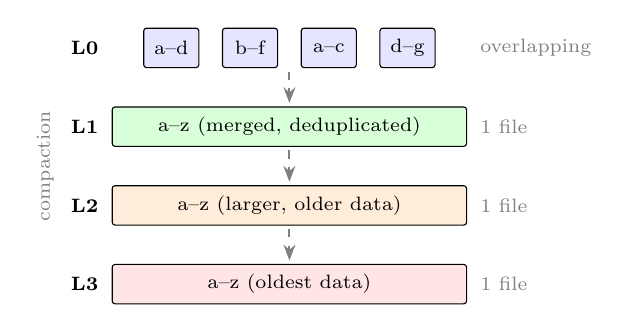
\begin{tikzpicture}[
    sst/.style={draw, fill=#1, minimum height=0.5cm, font=\scriptsize, rounded corners=1pt},
    arr/.style={-{Stealth[length=2mm]}, thick, dashed, gray},
    >=Stealth
]
% L0
\node[font=\scriptsize\bfseries, anchor=east] at (-0.8, 3.0) {L0};
\node[sst=blue!10, minimum width=0.7cm] at (0, 3.0) {a--d};
\node[sst=blue!10, minimum width=0.7cm] at (1.0, 3.0) {b--f};
\node[sst=blue!10, minimum width=0.7cm] at (2.0, 3.0) {a--c};
\node[sst=blue!10, minimum width=0.7cm] at (3.0, 3.0) {d--g};
\node[font=\scriptsize, gray, anchor=west] at (3.8, 3.0) {overlapping};

% L1
\node[font=\scriptsize\bfseries, anchor=east] at (-0.8, 2.0) {L1};
\node[sst=green!15, minimum width=4.5cm] at (1.5, 2.0) {a--z (merged, deduplicated)};
\node[font=\scriptsize, gray, anchor=west] at (3.8, 2.0) {1 file};

% L2
\node[font=\scriptsize\bfseries, anchor=east] at (-0.8, 1.0) {L2};
\node[sst=orange!15, minimum width=4.5cm] at (1.5, 1.0) {a--z (larger, older data)};
\node[font=\scriptsize, gray, anchor=west] at (3.8, 1.0) {1 file};

% L3
\node[font=\scriptsize\bfseries, anchor=east] at (-0.8, 0.0) {L3};
\node[sst=red!10, minimum width=4.5cm] at (1.5, 0.0) {a--z (oldest data)};
\node[font=\scriptsize, gray, anchor=west] at (3.8, 0.0) {1 file};

% Compaction arrows
\draw[arr] (1.5, 2.7) -- (1.5, 2.3);
\draw[arr] (1.5, 1.7) -- (1.5, 1.3);
\draw[arr] (1.5, 0.7) -- (1.5, 0.3);

\node[font=\scriptsize, gray, rotate=90] at (-1.6, 1.5) {compaction};

\end{tikzpicture}
\caption{KiwiDB level model. L0 uses tiering (multiple overlapping files). L1--L3 use leveling (one merged file per level). Compaction merges all L0 files into L1 when file count $\geq$ threshold.}
\label{fig:compaction}
\end{figure}

\textbf{Trigger mechanism.} Compaction is flush-triggered, not daemon-driven. After every flush commit, \texttt{CompactionManager.check\_and\_compact()} runs. Table~\ref{tab:compaction-triggers} shows the thresholds.

\begin{table}[t]
\centering
\caption{Compaction trigger thresholds.}
\label{tab:compaction-triggers}
\begin{tabular}{@{}lll@{}}
\toprule
\textbf{Transition} & \textbf{Trigger} & \textbf{Default} \\
\midrule
L0 $\rightarrow$ L1 & File count $\geq$ threshold & 10 files \\
L1 $\rightarrow$ L2 & Size $\geq$ $10^2 \times$ base & Cascading \\
L2 $\rightarrow$ L3 & Size $\geq$ $10^3 \times$ base & Cascading \\
\bottomrule
\end{tabular}
\end{table}

\textbf{K-way merge.} The \texttt{KWayMergeIterator} merges $N$ sorted inputs via a min-heap keyed on \texttt{(key, -seq)}. For equal keys, the highest seq (newest) wins. This enables single-pass deduplication. Tombstones with \texttt{seq < seq\_cutoff} are garbage-collected; those above the cutoff are preserved to shadow values in deeper levels.

\textbf{Subprocess execution.} Each compaction job is a \texttt{CompactionTask} --- a frozen dataclass with only primitive fields (strings, integers) that can cross the subprocess boundary. The merge runs in a \texttt{ProcessPoolExecutor} subprocess with its own GIL. As shown in Table~\ref{tab:gil-impact}, this is the only way to achieve true parallelism for CPU-bound work in CPython.

\textbf{Atomic commit.} After the subprocess produces the new SSTable, the commit sequence is: (1)~register new reader, (2)~write manifest, (3)~mark old files for deletion (deferred by ref-count), (4)~update in-memory state, (5)~evict stale cache. Write locks on source and destination levels prevent reads from seeing inconsistent state.

\textbf{Write amplification analysis.} Table~\ref{tab:write-amp} compares the write amplification of the three strategies.

\begin{table}[t]
\centering
\caption{Write amplification comparison at flush time. $T$ = size ratio (default 10), $L$ = record size, $B$ = block size, $\phi$ = bloom FPR.}
\label{tab:write-amp}
\begin{tabular}{@{}lcc@{}}
\toprule
\textbf{Strategy} & \textbf{Write amp.\ (flush)} & \textbf{Read amp.\ (bloom checks)} \\
\midrule
LevelDB (leveling) & $O(T \times L/B)$ & $L \times \phi = 0.04$ \\
KiwiDB (hybrid) & $O(L/B)$ & $T\phi + L\phi = 0.13$ \\
\midrule
\textbf{Improvement} & $\mathbf{10\times}$ & $3.25\times$ worse \\
\bottomrule
\end{tabular}
\end{table}

KiwiDB's L0 tiering eliminates the merge at flush --- a pure sequential append. The trade-off is checking up to $T$ bloom filters at L0 per read. With 1\% FPR: $10 \times 0.01 + 3 \times 0.01 = 0.13$ expected false positives per lookup, versus LevelDB's $3 \times 0.01 = 0.03$. This $3{-}4\times$ read cost increase is acceptable given the $10\times$ write improvement.

\subsection{SSTable Manager and Manifest}

The \texttt{SSTableManager} coordinates all on-disk state via a persistent JSON manifest:

\begin{lstlisting}[caption={Manifest structure.},label={lst:manifest}]
{
  "l0_order": ["file_a", "file_b"],
  "levels": {"1": "file_c", "2": "file_d"}
}
\end{lstlisting}

The \texttt{l0\_order} list stores file IDs in newest-first order. Per-level \texttt{AsyncRWLock} instances serialize compaction commits while allowing concurrent readers. A reference-counted registry prevents reader closure while in-flight reads are active. The manifest is written atomically via \texttt{tempfile} + \texttt{os.replace()}.

\subsection{Recovery Model}

On startup, KiwiDB reconstructs state in six steps:

\begin{enumerate}[leftmargin=*]
    \item Load config and open WAL file.
    \item Load all SSTables from disk via manifest. Directories without \texttt{meta.json} are discarded (incomplete writes).
    \item Compute \texttt{max\_seq} across all loaded SSTables.
    \item Replay WAL entries where \texttt{seq > max\_seq} into a fresh memtable.
    \item Restore \texttt{SeqGenerator} to \texttt{max\_seq}.
    \item Start flush pipeline and compaction manager.
\end{enumerate}

Entries already flushed to SSTables are skipped. The WAL is the source of truth for unflushed data.

\subsection{Observability Layer}

Figure~\ref{fig:observability} shows the observability architecture.

% --- Figure 9: Observability ---
\begin{figure}[t]
\centering
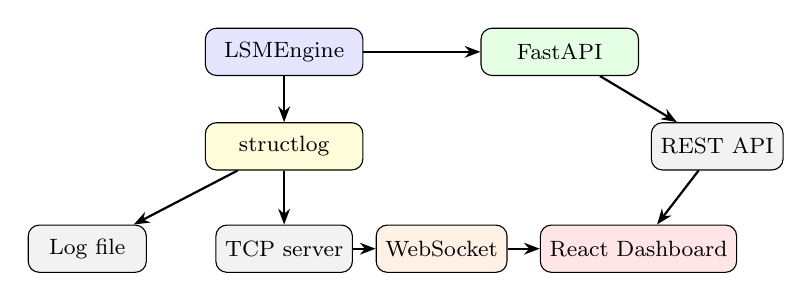
\begin{tikzpicture}[
    box/.style={draw, rounded corners, minimum width=2cm, minimum height=0.6cm, font=\footnotesize, fill=#1},
    arr/.style={-{Stealth[length=2mm]}, thick},
    >=Stealth
]
% Engine
\node[box=blue!10] (engine) at (0, 2.5) {LSMEngine};

% structlog
\node[box=yellow!15] (slog) at (0, 1.3) {structlog};
\draw[arr] (engine) -- (slog);

% File log
\node[box=gray!10, minimum width=1.5cm] (file) at (-2.5, 0) {Log file};
\draw[arr] (slog) -- (file);

% TCP broadcast
\node[box=gray!10, minimum width=1.5cm] (tcp) at (0, 0) {TCP server};
\draw[arr] (slog) -- (tcp);

% FastAPI
\node[box=green!10] (api) at (3.5, 2.5) {FastAPI};
\draw[arr] (engine) -- (api);

% REST
\node[box=gray!10, minimum width=1.5cm] (rest) at (5.5, 1.3) {REST API};
\draw[arr] (api) -- (rest);

% WebSocket
\node[box=orange!10, minimum width=1.5cm] (ws) at (2, 0) {WebSocket};
\draw[arr] (tcp) -- (ws);

% Dashboard
\node[box=red!10, minimum width=1.5cm] (dash) at (4.5, 0) {React Dashboard};
\draw[arr] (rest) -- (dash);
\draw[arr] (ws) -- (dash);

\end{tikzpicture}
\caption{Observability architecture. The engine emits structured logs to file and a TCP broadcast server. FastAPI exposes a REST API. The React dashboard consumes both REST endpoints and live WebSocket log streams.}
\label{fig:observability}
\end{figure}

\textbf{Structured logging.} All engine events are logged via \texttt{structlog} with key-value fields (seq, file\_id, level, size). Logs go to both a rotating file and a TCP broadcast server.

\textbf{REST API.} FastAPI exposes 20+ endpoints: KV operations (\texttt{GET/POST/DELETE /kv/\{key\}}), memtable inspection, SSTable browsing by level, engine statistics with history, configuration management, and a terminal interface.

\textbf{Web dashboard.} A React SPA (Vite + TypeScript) provides real-time views of memtable fill level, SSTable layout, compaction progress, live log stream, and an in-browser REPL.

\textbf{Live streaming.} The TCP log server relays events to WebSocket clients. Updates arrive without polling.

% ============================================================
\section{Implementation-Specific Details}
\label{sec:impl-details}
% ============================================================

In this section we discuss techniques specific to implementing an LSM engine in Python 3.12+.

\subsection{Async/Sync Bridge}

The engine uses three bridge patterns:

\begin{enumerate}[leftmargin=*]
    \item \textbf{Direct sync:} Microsecond operations (seq generation, memtable insert) execute synchronously inside an \texttt{async def} method.
    \item \textbf{\texttt{asyncio.to\_thread()}:} Blocking I/O (WAL fsync, mmap reads) is offloaded to the thread pool.
    \item \textbf{\texttt{ProcessPoolExecutor}:} CPU-bound compaction runs in a subprocess.
\end{enumerate}

\subsection{Sync-to-Async Signal Bridging}

When a sync write triggers a memtable freeze, the async flush pipeline must wake immediately. KiwiDB bridges this via \texttt{loop.call\_soon\_threadsafe()}: the sync code schedules an \texttt{asyncio.Event.set()} on the event loop, waking the pipeline on the next iteration. No polling; sub-millisecond latency.

\subsection{Writer-Preferred AsyncRWLock}

KiwiDB implements a custom \texttt{AsyncRWLock} with writer preference: once a writer is waiting, new readers block. This prevents writer starvation --- critical for compaction commits. The lock tracks three counters: active readers, active writers (0 or 1), and waiting writers.

\subsection{Backpressure}

When the immutable queue reaches capacity (default: 4), writes block via \texttt{threading.Event} with a 60-second timeout. If flush is stuck, a \texttt{FreezeBackpressureTimeout} exception is raised rather than allowing unbounded memory growth.

\subsection{Runtime-Mutable Configuration}

All parameters are stored in a thread-safe \texttt{Config} object backed by a JSON file. Values are read at point of use (not cached), so changes take effect on the next operation. Writes use atomic \texttt{os.replace()}. Table~\ref{tab:config} lists key parameters.

\begin{table}[t]
\centering
\caption{Key runtime-mutable configuration parameters.}
\label{tab:config}
\begin{tabular}{@{}llll@{}}
\toprule
\textbf{Parameter} & \textbf{Dev} & \textbf{Prod} & \textbf{Purpose} \\
\midrule
\texttt{max\_memtable\_entries} & 10 & --- & Freeze (count) \\
\texttt{max\_memtable\_size\_mb} & --- & 64 & Freeze (bytes) \\
\texttt{l0\_compact\_threshold} & 10 & 10 & L0 file limit \\
\texttt{bloom\_fpr} & 0.05 & 0.01 & Bloom FPR \\
\texttt{flush\_max\_workers} & 2 & 2 & Parallel flushes \\
\texttt{block\_size} & 4096 & 4096 & SSTable block (B) \\
\texttt{max\_levels} & 3 & 3 & Compaction depth \\
\bottomrule
\end{tabular}
\end{table}

\subsection{Type Safety and Formal Contracts}

Two independent type checkers run in strict mode on every CI check: \textbf{mypy} (disallows implicit \texttt{Any}) and \textbf{basedpyright} (additional flow analysis). Formal contracts are defined via ABCs (\texttt{StorageEngine}, \texttt{Serializable}, \texttt{MemTable}), Protocols (structural subtyping), and \texttt{.pyi} stub files for the public API.

% ============================================================
\section{Related Work}
\label{sec:related}
% ============================================================

\textbf{LSM tree foundations.} The LSM tree was proposed by O'Neil et al.~\cite{oneil1996} as a write-optimized alternative to B-trees. Luo and Carey~\cite{luo2020} formalized the design space across tiering, leveling, size ratio, and merge policy.

\textbf{Production implementations.} LevelDB~\cite{leveldb} is the canonical LSM implementation with pure leveling, a single compaction thread, and a global-mutex skip list. RocksDB~\cite{rocksdb} extends it with concurrent compaction, column families, and configurable strategies. WiredTiger~\cite{wiredtiger} combines B-tree and LSM approaches. All expose synchronous APIs.

\textbf{LSM on flash storage.} Wang et al.~\cite{wang2014locs} proposed LOCS, which extends LevelDB to exploit the channel-level parallelism of open-channel SSDs by increasing the number of Immutable MemTables and flushing them concurrently to separate channels. Their work demonstrates up to $4\times$ throughput improvement with optimized I/O scheduling. KiwiDB shares the insight that concurrent flush improves throughput, but achieves it at the software level with an event-chain commit ordering mechanism on commodity storage.

\textbf{Write amplification.} Dostoevsky~\cite{dayan2018} introduces lazy leveling as a hybrid between tiering and leveling. KiwiDB's L0-tiering / L1-leveling achieves a similar reduction through a simpler design.

\textbf{Bloom filter optimization.} Monkey~\cite{dayan2017} optimizes bloom filter memory across levels. KiwiDB instead sizes each filter from actual data, producing optimal filters without cross-level tuning.

\textbf{Concurrent data structures.} KiwiDB's skip list draws on Herlihy et al.~\cite{herlihy2006}, adapted for CPython's GIL: per-node locks for writers, GIL-atomic flag reads for lock-free readers.

% ============================================================
\section{Conclusion}
\label{sec:conclusion}
% ============================================================

We presented KiwiDB, a complete LSM tree key-value store built from scratch in Python~3.12+. By implementing the engine with an async-native API, parallel flush pipeline with event-chain commit ordering, and subprocess compaction for GIL bypass, we demonstrate that a modern storage engine can be built from first principles in a high-level language while incorporating design innovations that address real limitations in LevelDB and RocksDB.

The hybrid L0-tiering / L1-leveling strategy reduces write amplification by $10\times$ at the cost of $3.25\times$ more bloom filter checks --- an acceptable trade-off. The concurrent skip list achieves lock-free reads via GIL-atomic flag checks, and the three-tier block cache keeps hot bloom filters and indexes resident.

\textbf{Limitations.} KiwiDB trades feature breadth for depth: no range queries (though the internal merge iterator could support them), no block compression, no multi-key transactions, and $10{-}100\times$ lower raw throughput than C++ engines.

\textbf{Future work.} Natural extensions include: (1)~range query API exposing the merge iterator; (2)~LZ4/zstd block compression; (3)~WAL group commit for batched fsync; (4)~cross-level bloom optimization following Monkey~\cite{dayan2017}; (5)~migration to GIL-free Python (PEP~703) to replace subprocess compaction with true multi-threaded parallelism.

% ============================================================
% References
% ============================================================

\begin{thebibliography}{00}

\bibitem{oneil1996}
P.~O'Neil, E.~Cheng, D.~Gawlick, and E.~O'Neil, ``The log-structured merge-tree (LSM-tree),'' \textit{Acta Informatica}, vol.~33, no.~4, pp.~351--385, 1996.

\bibitem{leveldb}
Google, ``LevelDB: A fast and lightweight key/value database library,'' 2011. [Online]. Available: \url{https://github.com/google/leveldb}

\bibitem{rocksdb}
Facebook, ``RocksDB: A persistent key-value store for fast storage environments,'' 2013. [Online]. Available: \url{https://rocksdb.org}

\bibitem{cassandra}
A.~Lakshman and P.~Malik, ``Cassandra: A decentralized structured storage system,'' \textit{ACM SIGOPS Oper.\ Syst.\ Rev.}, vol.~44, no.~2, pp.~35--40, 2010.

\bibitem{chang2008}
F.~Chang, J.~Dean, S.~Ghemawat, W.~C.~Hsieh, D.~A.~Wallach, M.~Burrows, T.~Chandra, A.~Fikes, and R.~E.~Gruber, ``Bigtable: A distributed storage system for structured data,'' \textit{ACM Trans.\ Comput.\ Syst.}, vol.~26, no.~2, pp.~4:1--4:26, 2008.

\bibitem{decandia2007}
G.~DeCandia, D.~Hastorun, M.~Jampani, G.~Kakulapati, A.~Lakshman, A.~Pilchin, S.~Sivasubramanian, P.~Vosshall, and W.~Vogels, ``Dynamo: Amazon's highly available key-value store,'' in \textit{Proc.\ ACM SOSP}, 2007, pp.~205--220.

\bibitem{hbase}
Apache, ``HBase,'' [Online]. Available: \url{https://hbase.apache.org}

\bibitem{wiredtiger}
MongoDB, ``WiredTiger storage engine,'' [Online]. Available: \url{https://source.wiredtiger.com}

\bibitem{bloom1970}
B.~H.~Bloom, ``Space/time trade-offs in hash coding with allowable errors,'' \textit{Commun.\ ACM}, vol.~13, no.~7, pp.~422--426, 1970.

\bibitem{dayan2017}
N.~Dayan, M.~Athanassoulis, and S.~Idreos, ``Monkey: Optimal navigable key-value store,'' in \textit{Proc.\ ACM SIGMOD}, 2017, pp.~79--94.

\bibitem{dayan2018}
N.~Dayan and S.~Idreos, ``Dostoevsky: Better space-time trade-offs for LSM-tree based key-value stores via adaptive removal of superfluous merging,'' in \textit{Proc.\ ACM SIGMOD}, 2018, pp.~505--520.

\bibitem{herlihy2006}
M.~Herlihy, Y.~Lev, V.~Luchangco, and N.~Shavit, ``A provably correct scalable concurrent skip list,'' in \textit{Proc.\ OPODIS}, 2006.

\bibitem{luo2020}
C.~Luo and M.~J.~Carey, ``LSM-based storage techniques: A survey,'' \textit{The VLDB Journal}, vol.~29, pp.~393--418, 2020.

\bibitem{wang2014locs}
P.~Wang, G.~Sun, S.~Jiang, J.~Ouyang, S.~Lin, C.~Zhang, and J.~Cong, ``An efficient design and implementation of LSM-tree based key-value store on open-channel SSD,'' in \textit{Proc.\ ACM EuroSys}, 2014, pp.~16:1--16:14.

\bibitem{leavitt2010}
N.~Leavitt, ``Will NoSQL databases live up to their promise?'' \textit{Computer}, vol.~43, no.~2, pp.~12--14, 2010.

\bibitem{python-gil}
Python Software Foundation, ``GlobalInterpreterLock,'' [Online]. Available: \url{https://wiki.python.org/moin/GlobalInterpreterLock}

\end{thebibliography}

\end{document}
